\documentclass[../main.tex]{subfiles}

\begin{document}


\chapter{安装}
\vspace{-2cm}


本章节首先介绍了安装 BasicSR 所需的环境依赖\ref{section: env reqirement},随后介绍了安装 BasicSR 的两种方式\ref{section: install}:本地 clone 安装和 pip 安装。对于需要在项目中使用 PyTorch C++ 扩展的情况,我们也提供了相应的安装方式\ref{section:c++}。最后,我们将安装过程中有可能会遇到的一些问题进行了汇总\ref{section:question}。

\section{环境依赖}
\label{section: env reqirement}

由于 BasicSR 是基于 \href{https://www.python.org/}{Python} 语言和 \href{https://pytorch.org/}{PyTorch} 深度学习框架进行开发的,因此在安装 BasicsR 之前,需要在电脑或者服务器上安装 Python 环境以及各种相关的 Python 库;如果想要在\textbf{GPU}上运行程序的话,也需要先在电脑上配置相应的CUDA环境。以下我们分别对 CUDA 和相应的 Python 库进行简要的说明。

\begin{enumerate}
    \item NVIDIA GPU + \href{https://developer.nvidia.com/cuda-downloads}{CUDA}:GPU (Graphics Processing Unit) 由于其高效的并行能力,目前被广泛用于深度学习的计算当中;CUDA (Compute Unified Device Architecture) 是显卡厂商 NVIDIA 推出的可以让 GPU 解决复杂的计算问题的运算平台。如果需要训练 BasicSR 中的模型,推荐使用 GPU 并配置好相应的 CUDA 环境。

    \item Python 和 Python 库 (对于 Python 库,我们提供了相应的安装脚本):
    \begin{enumerate}
        \item Python >= 3.7 (推荐使用\href{https://www.anaconda.com/products/distribution#linux}{Anaconda}或者\href{https://docs.conda.io/en/latest/miniconda.html}{Miniconda})
        \item \href{https://pytorch.org/}{PyTorch >= 1.7}:目前深度学习领域广泛使用的深度学习框架。
        \item \href{https://pytorch.org/}{Torchvision >= 0.9.0}:Pytorch 的一个图形库,它服务于 PyTorch 深度学习框架的,主要用来构建计算机视觉模型。
    \end{enumerate}
\end{enumerate}

当配置好 Python 环境和 CUDA 环境之后,可以直接运行以下的脚本一次性安装 BasicSR 中调用的各种 Python 库:

    \begin{minted}[xleftmargin=20pt,bgcolor=bg]{python}
pip install -r requirements.txt
    \end{minted}



\section{BasicSR 安装}
\label{section: install}
在安装好上述的环境依赖后,此时就可以进行 BasicSR 的安装了。

\begin{hl} % ---------------- Highlight block ---------------- %
	\textbf{BasicSR 安装选项}

	根据不同的需求,我们提供了两种安装 BasicSR 方式,\textbf{两种方式只能选择一种安装}。
	\begin{itemize}
		\item 如果希望去\textbf{探究 BasicSR 中的细节}或者需要对其进行\textbf{修改},推荐通过本地 clone 的方式进行安装。
		\item 如果仅仅是将 BasicSR 作为一个\textbf{功能包}进行使用 (如 \href{https://github.com/TencentARC/GFPGAN}{GFPGAN},\href{https://github.com/xinntao/Real-ESRGAN}{Real-ESRGAN}),推荐直接从 PyPI 安装 BasicSR,这样可以使得自身项目的代码结构更加简洁。
	\end{itemize}
\end{hl}

\subsection{本地 clone}
\label{subsection:pip-install}
要通过本地 clone 安装 BasicSR,需要在终端上依次进行以下3个步骤。

\begin{enumerate}
    \item 克隆项目:
    \begin{minted}[xleftmargin=20pt,bgcolor=bg]{python}
git clone https://github.com/XPixelGroup/BasicSR.git
    \end{minted}

    \item 安装依赖包:
    \begin{minted}[xleftmargin=20pt,bgcolor=bg]{python}
cd BasicSR
pip install -r requirements.txt
    \end{minted}

    \item 安装 BasicSR:(此时在 BasicSR 的根目录下)

    \begin{minted}[xleftmargin=20pt,bgcolor=bg]{python}

python setup.py develop

    \end{minted}

%     \begin{enumerate}
%     \item 如果不需要使用 PyTorch C++ 扩展:(参考\ref{section:env})
%     \begin{minted}[xleftmargin=20pt,bgcolor=bg]{python}

% python setup.py develop

%     \end{minted}

%     \item 如果仅仅希望即时加载 PyTorch C++ 扩展 :
%     \begin{minted}[xleftmargin=20pt,bgcolor=bg]{python}

% python setup.py develop

%     \end{minted}
%     \item 如果在安装的时候希望编译 PyTorch C++ 扩展,此时需要设置环境变量:
%     \begin{minted}[xleftmargin=20pt,bgcolor=bg]{python}

% BASICSR_EXT=True python setup.py develop

%     \end{minted}
% \end{enumerate}


\end{enumerate}

\label{section:clone}



如果希望安装的时候指定 CUDA 路径,可以输入如下指令:

\begin{minted}[xleftmargin=20pt,bgcolor=bg]{python}

CUDA_HOME=/usr/local/cuda \
CUDNN_INCLUDE_DIR=/usr/local/cuda \
CUDNN_LIB_DIR=/usr/local/cuda \
python setup.py develop

\end{minted}

\subsection{pip 安装}
\label{subsection:pip-install}
对于使用 pip 安装 BasicSR,在终端上运行以下指令即可:
    \begin{minted}[xleftmargin=20pt,bgcolor=bg]{python}

pip install basicsr

    \end{minted}

% 我们提供了以下三种安装选项。

% \begin{enumerate}
%     \item 如果项目中不涉及 PyTorch C++ 扩展:
%     \begin{minted}[xleftmargin=20pt,bgcolor=bg]{python}

% pip install basicsr

%     \end{minted}

%     \item 如果仅仅希望即时加载 PyTorch C++ 扩展: (参考\ref{section:env})
%     \begin{minted}[xleftmargin=20pt,bgcolor=bg]{python}

% pip install basicsr

%     \end{minted}

%     \item 如果在安装的时候希望编译 PyTorch C++ 扩展,此时需要设置环境变量:

%     \begin{minted}[xleftmargin=20pt,bgcolor=bg]{python}

% BASICSR_EXT=True pip install basicsr

%     \end{minted}

%     \begin{note} % ---------------- Note block ---------------- %
%     	\textbf{注意}

%     	如果安装失败,报错信息为 \textit{ImportError: cannot import name 'deform\_conv\_ext', 'fused\_act\_ext', 'upfirdn2d\_ext'},此时需要重新安装,并输入以下指令从而在安装的时候获取详尽的日志:

%     	\begin{minted}[xleftmargin=20pt,bgcolor=bg]{python}

% BASICSR_EXT=True pip install basicsr -vvv

%         \end{minted}

%     \end{note}

% \end{enumerate}


如果希望安装的时候指定 CUDA 路径,可以输入如下指令:

\begin{minted}[xleftmargin=20pt,bgcolor=bg]{python}

CUDA_HOME=/usr/local/cuda \
CUDNN_INCLUDE_DIR=/usr/local/cuda \
CUDNN_LIB_DIR=/usr/local/cuda \
pip install basicsr

\end{minted}

\subsection{检验 BasicSR 是否安装成功}

当选择了上述两种方式中的一种方式安装 BasicSR 时,我们可以通过图\ref{fig:correct-install}的方式来判断是否成功安装 BasicSR:

    \begin{figure}[H]
	%\vspace{-0.5cm}
	\begin{center}
		%\fbox{\rule{0pt}{2.5in} \rule{0.9\linewidth}{0pt}}
		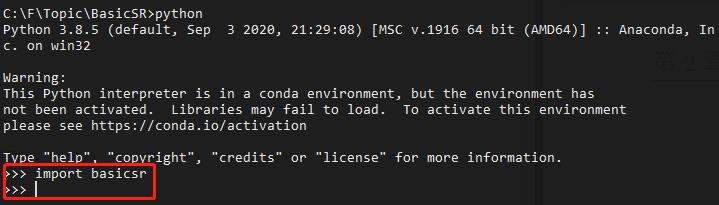
\includegraphics[width=0.8\linewidth]{figures/installation_correct_install.jpg}
		\caption{成功安装 BasicSR}
		\label{fig:correct-install}
	\end{center}
	\vspace{-0.5cm}
    \end{figure}

如果此时没有报错,则说明 BasicSR 安装成功,此时便可以基于 BasicSR 进行开发啦 $\sim \sim \sim$

% \section{BASICSR\_EXT 和 BASICSR\_JIT 环境变量介绍}

\section{PyTorch C++ 扩展使用}
\label{section:c++}

\begin{note} % ---------------- Highlight block ---------------- %

	考虑到某些项目中会需要使用 PyTorch C++ 扩展,我们在这个小节针对这种情况也提供了相应的 BasicSR 安装方式。如果不需要使用相关 C++ 扩展,则此小节可以跳过。
\end{note}

对于项目中需要使用以下的 PyTorch C++ 扩展时,具体为以下两种情况:

\begin{itemize}
    \item 可变性卷积 (如果安装的 Torchvision 版本 >= 0.9.0,可跳过):\href{https://github.com/XPixelGroup/BasicSR/tree/master/basicsr/ops}{EDVR 中的 DCN}

    \item StyleGAN 中的特定的算子:\href{https://github.com/XPixelGroup/BasicSR/tree/master/basicsr/ops}{upfirdn2d, fused\_act}
\end{itemize}

由于\ref{section: install}所提到的安装方式不支持 PyTorch C++ 扩展,为了能够使用 PyTorch C++ 扩展,此时需要一些特定的修改 (有以下两种方式可供选择):


\begin{enumerate}
    \item \textbf{安装}的时候对 PyTorch C++ 扩展进行编译:此时需要将原先的安装指令进行修改,
    \begin{enumerate}
        \item 对于通过本地 clone 安装 BasicSR 的方式,此时修改指令:
        \begin{minted}[xleftmargin=20pt,bgcolor=bg]{python}
python setup.py develop --> BASICSR_EXT=True python setup.py develop
        \end{minted}
        \item 对于通过 pip 安装 BasicSR 的方式,此时修改指令:
        \begin{minted}[xleftmargin=20pt,bgcolor=bg]{python}
pip install basicsr --> BASICSR_EXT=True pip install basicsr
        \end{minted}
    \end{enumerate}
    当进行了上述的修改之后,如果我们需要运行 StyleGAN 的测试代码 (位于inference/inference\_stylegan2.py),此时直接输入指令即可:
    \begin{minted}[xleftmargin=20pt,bgcolor=bg]{python}
python inference/inference_stylegan2.py
        \end{minted}

    \item \textbf{每次在跑程序}的时候\textbf{即时加载 (JIT)} PyTorch C++ 扩展:如果我们选择了这种方式,此时不需要修改 BasicSR 的安装指令。依然拿 StyleGAN 的测试代码举例,在这种情况下,如果想要运行 StyleGAN 的测试代码,此时需要输入的指令是:
    \begin{minted}[xleftmargin=20pt,bgcolor=bg]{python}
BASICSR_JIT=True python inference/inference_stylegan2.py
    \end{minted}

\end{enumerate}


关于上述提到的两种使用 PyTorch C++ 扩展方式之间的优劣即场景对比如表\ref{tab:env}所示:

\begin{table}[h]
\centering
\footnotesize
\begin{tabular}{|c|c|c|c|c|}
%   \hline
%   \multicolumn{5}{|c|}{BASICSR\_EXT和BASICSR\_JIT环境变量的对比} \\
  \hline
  选项                     & 优点                  & 缺点                            & 适用场景         & 具体安装指令 \\
  \hline
  安装编译 C++ 扩展 & \makecell[c]{运行代码的时候, \\ 能够快速加载扩展} & \makecell*[c]{配置环境的时候, \\ 需要更多的依赖,\\碰到的问题可能更多} & \makecell[c]{需要多次训练 \\ 或者测试模型} & \makecell[c]{在安装的时候,设置 \\\textbf{BASICSR\_EXT=True}}\\
  \hline
  即时加载 C++ 扩展 & \makecell[c]{有着更少的依赖,\\碰到的问题可能更少} & \makecell[c]{每次运行代码的时候,\\都需要花费几分钟\\重新加载扩展} & 仅仅是进行测试 & \makecell[c]{在跑程序的时候,设置 \\\textbf{BASICSR\_JIT=True}} \\
  \hline
\end{tabular}
\caption{\label{tab:env}安装编译扩展和即时加载扩展的对比。}
\end{table}


\begin{note} % ---------------- Note block ---------------- %
    \textbf{注意}
	\begin{enumerate}
	    \item 对于需要在安装的时候就编译 PyTorch C++ 扩展,需要确保:gcc 和 g++ 版本 >= 5。
	    \item BasicSR\_JIT 有最高的优先级。即使在安装的时候已经成功编译了 C++ 扩展,如果在运行代码指令中设置了 BasicSR\_JIT=True,此时代码会即时加载 C++ 扩展。
	    \item 在\textbf{安装}的时候,不能设置 BasicSR\_JIT=True。
	\end{enumerate}
\end{note}




\section{常见问题}
\label{section:question}


\begin{enumerate}
    \item \textbf{Q1: Windows 下是否可以使用?}

    经过验证,Windows 下可以通过上述的两种安装方式安装 BasicSR 的 CPU 版本。如果需要使用 CUDA,需要指定 CUDA 路径。由于 BasicSR 项目是在 Linux 环境下进行开发的,因此推荐在 Linux 环境下基于 BasicSR 进行项目的开发。

    \item \textbf{Q2: BASICSR\_EXT 和 BASICSR\_JIT 在什么环境下才能执行?}

    如果在加入 BASICSR\_EXT 和 BASICSR\_JIT 环境变量之后运行报错,此时需要检测 gcc 版本。BasicSR 在已被验证在 gcc5 $\sim$ gcc7 版本下可以成功编译 C++ 扩展。

    \item \textbf{Q3: 是否可以同时使用上面提到的两种方式 (clone 和 pip) 安装了 BasicSR?}

    上述两种安装方式只能选择一种进行安装,安装两个会存在路径混淆问题。具体而言,如果我们先通过 pip 安装了 BasicSR,如果我们随后又使用本地 clone 的方式进行安装,此时项目中调用的 BasicSR 路径还是 pip 安装的 BasicSR;反过来,如果先使用本地 clone 的方式进行安装,随后又使用 pip 安装,此时项目中调用的 BasicSR 路径还是本地 clone 下的BasicSR (如图\ref{fig:false-clone-install}和图\ref{fig:false-pip-install})。

\begin{enumerate}
    \item 正常我们通过本地 clone 安装的时候,此时使用 pip list 查看此时 basicsr 路径:
    \begin{figure}[H]
	%\vspace{-0.5cm}
	\begin{center}
		%\fbox{\rule{0pt}{2.5in} \rule{0.9\linewidth}{0pt}}
		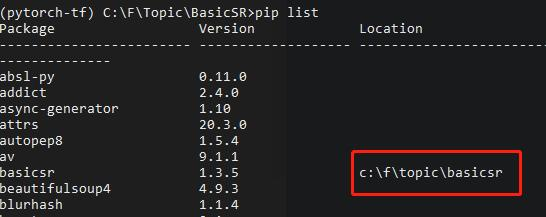
\includegraphics[width=0.5\linewidth]{figures/installation_clone_install_location.jpg}
		\caption{本地 clone 安装成功时的 basicsr 路径显示}
		\label{fig:correct-clone-install}
	\end{center}
	\vspace{-0.5cm}
    \end{figure}

    \item 正常我们通过 pip 安装的时候,此时使用 pip list 查看此时 basicsr 路径:
    \begin{figure}[H]
	%\vspace{-0.5cm}
	\begin{center}
		%\fbox{\rule{0pt}{2.5in} \rule{0.9\linewidth}{0pt}}
		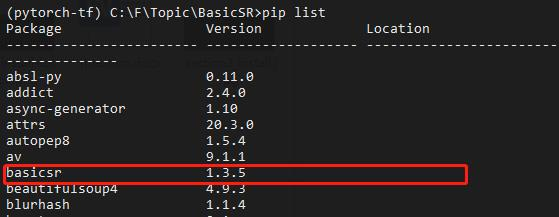
\includegraphics[width=0.5\linewidth]{figures/installation_pip_install_location.jpg}
		\caption{pip 安装成功时的 basicsr 路径显示 (如果指向 anaconda 下的路径,也是正常的)}
		\label{fig:correct-pip-install}
	\end{center}
	\vspace{-0.5cm}
    \end{figure}

    \item 如果先通过 pip 安装,随后通过本地 clone 安装,此时使用 pip list 查看 basicsr 路径:
    \begin{figure}[H]
	%\vspace{-0.5cm}
	\begin{center}
		%\fbox{\rule{0pt}{2.5in} \rule{0.9\linewidth}{0pt}}
		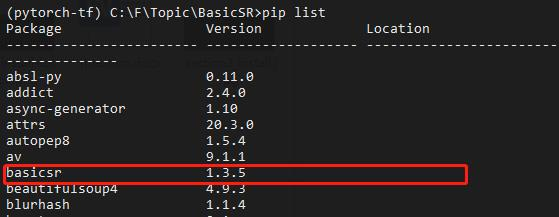
\includegraphics[width=0.5\linewidth]{figures/installation_pip_install_location.jpg}
		\caption{basicsr 路径并未指向本地 clone 的 BasicSR}
		\label{fig:false-clone-install}
	\end{center}
	\vspace{-0.5cm}
    \end{figure}

    \item 如果先通过本地 clone 安装,随后通过 pip 安装,通过 pip list 查看此时 basicsr 路径:
    \begin{figure}[H]
	%\vspace{-0.5cm}
	\begin{center}
		%\fbox{\rule{0pt}{2.5in} \rule{0.9\linewidth}{0pt}}
		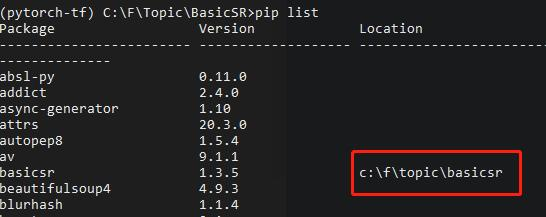
\includegraphics[width=0.5\linewidth]{figures/installation_clone_install_location.jpg}
		\caption{basicsr 路径并未指向 python 环境下 (或者 anaconda) 下 的 BasicSR}
		\label{fig:false-pip-install}
	\end{center}
	\vspace{-0.5cm}
    \end{figure}

\end{enumerate}


    对于上述的两种错误情况 (图\ref{fig:false-clone-install}和图\ref{fig:false-pip-install}),此时正常的解决方式为:
\begin{minted}[xleftmargin=20pt,bgcolor=bg]{python}

pip uninstall basicsr

\end{minted}

    先将安装的 BasicSR 进行卸载,随后再根据项目的需要重新选择一种方式安装 BasicSR。

    \item \textbf{Q4: 如何更新最新版本的 BasicSR?}

\begin{enumerate}
    \item 对于 clone 安装,需要将本地的 BasicSR 项目代码与\href{https://github.com/XPixelGroup/BasicSR}{远端的 BasicSR 项目代码}进行同步。
    \item 对于 pip 安装,需要先卸载当前版本的 BasicSR,再重新使用 pip 安装最新版本的 BasicSR。
\end{enumerate}

    \item \textbf{Q5: 如何解决运行代码时出现的 version 问题?}

    有时候在运行代码的时候,会出现类似于如下的问题:
    \begin{figure}[H]
	%\vspace{-0.5cm}
	\begin{center}
		%\fbox{\rule{0pt}{2.5in} \rule{0.9\linewidth}{0pt}}
		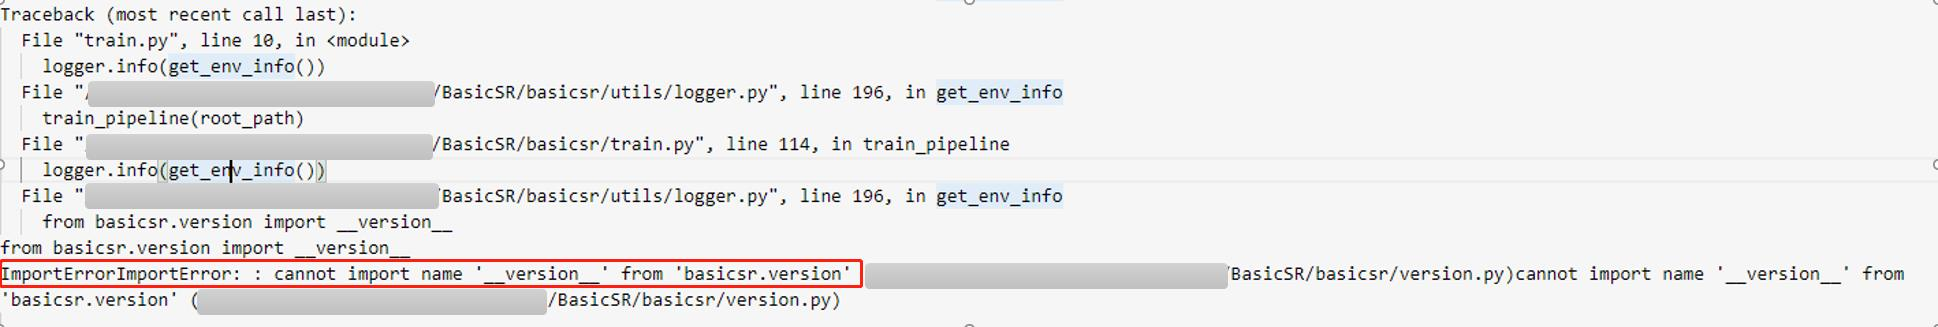
\includegraphics[width=0.8\linewidth]{figures/installation_version.jpg}
		\caption{version问题示例}
		\label{fig:version}
	\end{center}
	\vspace{-0.5cm}
    \end{figure}
    此时,可以尝试:
    \begin{enumerate}
        \item 重新运行安装 BasicSR 的指令。
        \item 将涉及到 version 的代码进行注释。
    \end{enumerate}

\end{enumerate}

\begin{hl}
    如果小伙伴们在安装过程中还遇到其它的问题,可以在我们的 BasicSR 微信群、 QQ 群 (可从 \href{https://github.com/XPixelGroup/BasicSR/blob/master/README_CN.md}{BasicSR 项目主页}中获取)、\href{https://github.com/XPixelGroup/BasicSR/issues}{github 的 issue} 上面进行反馈,我们会持续将一些常见的问题更新到这个小节当中。
\end{hl}


\end{document}